\documentclass[border=8pt,tikz]{standalone}
\usepackage{tikz}
% Shared TikZ style for Chapter 5 diagrams.
% Inputted by every standalone diagram file.

\usetikzlibrary{
  arrows.meta,
  positioning,
  shapes.geometric,
  shapes.symbols,
  shapes.multipart,
  shapes.misc,
  fit,
  calc,
  backgrounds,
  decorations.pathmorphing,
  decorations.pathreplacing,
  patterns,
  shadows.blur,
}

% ─── Colour palette ──────────────────────────────────────────────
\definecolor{strixBlue}{HTML}{3B7DD8}     % data sources / inputs
\definecolor{strixGreen}{HTML}{22A699}    % processing / workers
\definecolor{strixOrange}{HTML}{E08036}   % storage
\definecolor{strixRed}{HTML}{E04B4B}      % attacker / external threat
\definecolor{strixPurple}{HTML}{6B5DD3}   % frontend / UI
\definecolor{strixGold}{HTML}{F2BE22}     % models / ML
\definecolor{strixGrey}{HTML}{6E7681}     % neutral / labels
\definecolor{strixDark}{HTML}{1F2933}     % titles / borders

% ─── Common node styles ──────────────────────────────────────────
\tikzset{
  >={Latex[width=2mm,length=2.5mm]},
  font=\sffamily\small,
  every node/.style={align=center},
  comp/.style={
    rectangle, rounded corners=2pt, draw=#1, fill=#1!10, very thick,
    text=strixDark, minimum width=22mm, minimum height=8mm,
    inner sep=4pt,
  },
  comp/.default=strixGreen,
  store/.style={
    cylinder, shape border rotate=90, aspect=0.3, draw=strixOrange,
    fill=strixOrange!12, very thick, text=strixDark,
    minimum width=18mm, minimum height=10mm, inner sep=2pt,
  },
  stream/.style={
    rectangle, rounded corners=2pt, draw=strixOrange,
    fill=strixOrange!8, dashed, thick, text=strixDark,
    minimum width=22mm, minimum height=7mm, inner sep=3pt,
    font=\ttfamily\scriptsize,
  },
  source/.style={comp=strixBlue},
  worker/.style={comp=strixGreen},
  model/.style={comp=strixGold},
  ui/.style={comp=strixPurple},
  ext/.style={comp=strixRed},
  title/.style={font=\sffamily\bfseries, text=strixDark},
  edge/.style={->, thick, draw=strixGrey, font=\sffamily\scriptsize\itshape},
  edgeStrong/.style={->, very thick, draw=strixDark, font=\sffamily\scriptsize\bfseries},
  group/.style={
    rectangle, rounded corners=4pt, draw=strixGrey, dashed, thick,
    inner sep=6pt, fill=strixGrey!4,
  },
  badge/.style={
    rectangle, rounded corners=1pt, fill=#1, text=white,
    font=\sffamily\scriptsize\bfseries, inner sep=2pt,
  },
  badge/.default=strixDark,
  port/.style={
    rectangle, rounded corners=1pt, draw=strixDark, fill=strixGrey!8,
    font=\ttfamily\scriptsize, minimum width=14mm, inner sep=2pt,
  },
}


\begin{document}
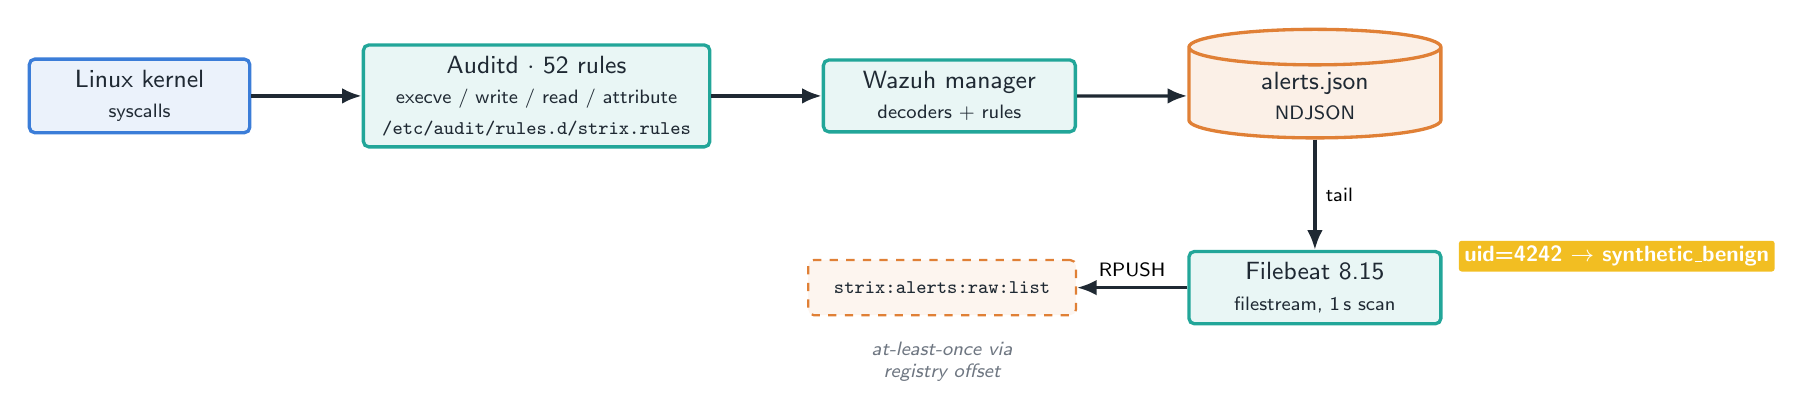
\begin{tikzpicture}[node distance=14mm]

\node[source, minimum width=28mm] (k) {Linux kernel\\\scriptsize syscalls};

\node[worker, right=of k, minimum width=44mm] (ad) {Auditd \(\cdot\) 52 rules\\
  \scriptsize execve / write / read / attribute\\\scriptsize \texttt{/etc/audit/rules.d/strix.rules}};

\node[worker, right=of ad, minimum width=32mm] (wm) {Wazuh manager\\\scriptsize decoders + rules};

\node[store, right=of wm, minimum width=32mm] (af)
  {alerts.json\\\scriptsize NDJSON};

\node[worker, below=of af, minimum width=32mm] (fb)
  {Filebeat 8.15\\\scriptsize filestream, 1\,s scan};

\node[stream, left=of fb, minimum width=34mm] (rl)
  {strix:alerts:raw:list};

\node[font=\sffamily\scriptsize\itshape, text=strixGrey, anchor=north]
  at ([yshift=-2mm]rl.south) {at-least-once via\\registry offset};

\draw[edgeStrong] (k) -- (ad);
\draw[edgeStrong] (ad) -- (wm);
\draw[edgeStrong] (wm) -- (af);
\draw[edgeStrong] (af) -- (fb) node[midway, right, font=\sffamily\scriptsize] {tail};
\draw[edgeStrong] (fb) -- (rl) node[midway, above, font=\sffamily\scriptsize] {RPUSH};

% Synthetic-benign annotation
\node[badge=strixGold, anchor=west]
  at ([xshift=2mm, yshift=4mm]fb.east) {\footnotesize uid=4242 \(\to\) synthetic\_benign};

\end{tikzpicture}
\end{document}
